\documentclass[a4paper]{article}
\usepackage[margin=1in]{geometry}
\usepackage{hyperref}
\usepackage{graphicx}
%opening
\title{Philosophy of Life Sciences.\\ On Reinfocement Learning and Compatibilism}
\author{Sergei Volodin, EPFL MSc student}
\date{}

\begin{document}

\maketitle

\begin{abstract}
Two seemingly unrelated concepts are considered, namely, Reinfocement Learning and Compatibilism. This paper claims that a new emerging paradigm in Artificial Intelligence, namely, Reinforcement Learning, can answer a question on whether or not free will is compatible with determinism (also known as compatibilism).
First, human behavior are linked with Reinforcement Learning paradigm using recent studies in Computer Science and Neuroscience.
After that, human behavior is analyzed in the RL framework and a few possible cases are considered. First of them leads to incompatibilism between free will and determinism.
\end{abstract}

\section{Introduction}
Free will is a philosophical concept stating that humans can choose between possible actions in a particular situation \cite{freewillst}. This notion has two possible views linked to it. First one states that free will does not exist, which means that actions of humans are not determined by themselves and no other action could have been taken rather than the one that actually happened. Second view states that free will exists. In any particular situation, regardless of the previous events, other action could have been chosen rather than the one that actually was.

Determinism \cite{determinismst} is the notion of events in the world being {\em caused} only by the previous ones, and not by anything else. In other words, if the world was in one particular state in the first moment of time $t_1$, it could only be in one state in the second moment of time $t_2>t_1$, and this state depends only on previous state.

Free will and determinism are often contrasted in a mutually exclusive manner. This idea is called Incompatibilism \cite{compatibilismst}. It claims that if there exist free will, the world cannot be deterministic, and vice versa. The opposite view is called compatibilism which states that these two concepts can be true together.

Reinforcement learning is a subfield of Machine Learning and Artificial Intelligence considering two entities: the {\em agent} and the {\em environment}. {\em Agent} is taking {\em actions} inside the {\em environment}, and the {\em environment} sends this agent back {\em observations}, which are states of the environment and {\em rewards}, which are numbers indicating how well the agent performs \cite{sutton}.

\begin{figure}[h]
	\caption{Reinforcement Learning diagram}
	\centering 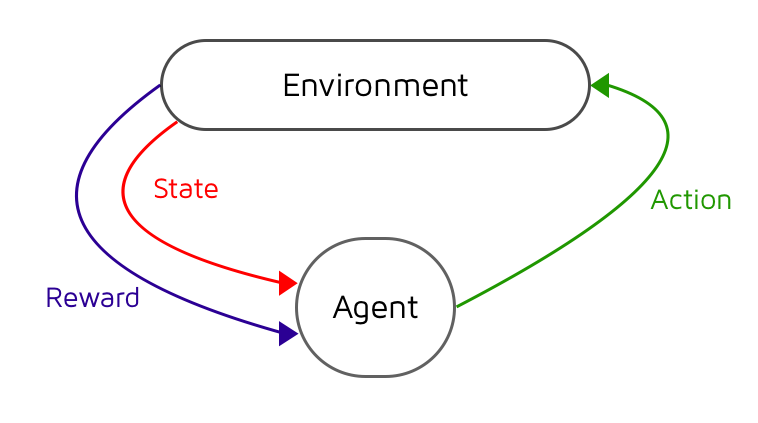
\includegraphics[width=150px]{RL.png}
	\label{RL}
\end{figure}

Recent studies in Neuroscience suggest that the brain of mammals, such as mice and monkeys, actually has structures in it which resemble parts of the Reinforcement Learning algorithms in its inner processing to generate actions \cite{doyareward, doya2}. Thus, it is plausible to assume that such a framework is also used in humans. Moreover, a philosophical view on Reinfocement Learning suggests that RL agents are no different from animals in terms of behavior, and, thus, might be considered conscious to some extent \cite{rlmorality1, rlmorality2}. When linking the reinfocement learning framework to human-world interaction, we will assume that humans possess Artificial General Intelligence \cite{shane}, meaning that a human can solve {\em any} task, if given enough time to do it. If the task can be solved in a finite time $t$, but not during the lifetime ($t>T$), we do not consider such a task.

First problem that this essay will address is the seemingly impossible existence of free will under the assumption of applicability of RL to humans. If the actions of humans can be explained by a mathematical model, if not in each case, then on average, how can humans might have free will? It shall be shown that reinforcement learning action selection requires randomness in most cases. For example, when choosing exploration or exploitation strategy \cite{sutton}, most of the agents use a source of random bits. Thus, a reinforcement learning algorithm does not depend solely on the observations and rewards given by the environment. It means that, given a history of interaction between environment and the agent to two different agents of the same type, they {\em can} produce different actions for the next input from the environment.

This randomness can come from both of the two entities, from the agent, and from the environment. If the randomness comes from the environment, then, in a deterministic world learning as we know it would not be possible, meaning that there would exist real-world situations which a randomness-equipped agent can solve, when a deterministic agent cannot. In this paragraph, learning denotes the ability of the agent to begin to act in a way to obtain maximal reward after some time of training.

An example of such situation would be the following. Consider an environment with two possible actions, for example, choosing a restaurant A or B. They have different menus and each of them has a certain amount of satisfaction (reward) associated to it. At the beginning the menus are the same, but at time steps $t$ in $t_1,...,t_n$ the restaurant B changes the menu and it now has higher reward associated to it (is more satisfactory). Suppose now that we have an agent who only chosen the A, and never took B. Regardless of the inner design of the agent, we can take into account the very first time he chooses the option B at $t'$. If $t'$ is not one of $t_1,...,t_n$, then he wouldn't see the difference at all, thus, he will never know that the restaurant B is better for him.

Continuing in this manner, for each agent we can construct the restaurants environment which is unsolvable for it, meaning that it has no chance of ever choosing B and obtaining higher reward, despite the fact that it was possible. Thus, for each possible agent we have constructed an environment which is unsolvable for it. This contradicts to the assumption of humans possessing AGI, which states that a human can solve any given task in finite time.

In case if the agent has randomness at his hand, we cannot talk about his actions as of deterministic quantities anymore. Despite all of the choices he made, he can just choose option B at any particular time, and the environment cannot be constructed as in the previous example. It means that there exist an agent which would have non-zero average visit count of restaurant B. For example, it can choose actions randomly each time. Then he would choose the action $B$ at $t_1$ in half of the cases and win.


On the other hand, if the randomness does not come from the environment itself, it can come from inside the agent, meaning that it is the agent who takes decisions of whether or not to explore. This case can be interpreted as a single instance of free choice. It is interpreted as follows: given two equally rewarding options to decide between, $a$ and $b$, and a action-value function \cite{sutton} $Q(s, a)=Q(s, b)$, meaning that the previous history suggests the agent that two actions are equally rewarding, the agent himself can choose which action to take, irregardless of the environment, by generating one bit using free will.

However, in the latter case the environment cannot be deterministic, since human mind is part of it, and it should be able to generate random bits. Otherwise, the same restaurant example can be constructed. Thus, in the latter case, if we assume that randomness comes from the agent itself, we must conclude that the world is not deterministic, thus, we obtain incompatibilism of free will and determinism, namely, free will holds, when determinism cannot be true.

Finally, this paper argues that the latter case is true. If the environment is the source of randomness, then an environment can be constructed which would give the exact bits to the agents that make the environment unsolvable.

\begin{thebibliography}{20}
\bibitem{freewillst} \url{https://plato.stanford.edu/entries/freewill/}
\bibitem{doyareward} Kazuyuki Samejima1, Yasumasa Ueda, Kenji Doya, Minoru Kimura. Representation of Action-Specific Reward Values in the Striatum
\bibitem{determinismst} \url{https://plato.stanford.edu/entries/determinism-causal/}
\bibitem{compatibilismst} \url{https://plato.stanford.edu/entries/compatibilism/}
\bibitem{doya2} K. Doya. What are the computations of the cerebellum, the basal ganglia and the cerebral cortex?
\bibitem{sutton} Richard S. Sutton and Andrew G. Barto. 1998. Introduction to Reinforcement Learning (1st ed.). MIT Press, Cambridge, MA, USA.
\bibitem{freewillrl} Kenneth T. Kishida. A computational approach to “free will” constrained by the games we play
\bibitem{rlmorality1} Brian Tomasik. Do Artificial Reinforcement-Learning Agents Matter Morally?
\bibitem{rlmorality2} \url{http://reducing-suffering.org/ethical-issues-artificial-reinforcement-learning/}
\bibitem{shane} Shane Legg. Machine Super Intelligence
%\bibitem{1} \url{http://oxfordindex.oup.com/view/10.1093/acprof:oso/9780198713241.003.0003}
%\bibitem{2} Negation of Free will: \url{//www.informationphilosopher.com/freedom/standard_argument.html}
%\bibitem{3} \url{https://plato.stanford.edu/entries/freewill/}
%\bibitem{4} \url{http://serendip.brynmawr.edu/sci_cult/evolit/s05/web2/lpaterek.html}
%\bibitem{5} \url{https://www.researchgate.net/publication/278468286_Creating_Free_Will_in_Artificial_Intelligence}
%\bibitem{6} \url{https://philosophy.stackexchange.com/questions/36639/in-what-type-of-world-is-free-will-possible-if-at-all}
%\bibitem{7} \url{https://becominghuman.ai/can-a-i-ever-have-free-will-c18b4f489b45}
%\bibitem{8} \url{https://philpapers.org/browse/philosophy-of-artificial-intelligence}
%\bibitem{9} \url{https://en.wikipedia.org/wiki/Philosophy_of_artificial_intelligence}
%\bibitem{a} \url{https://www.theguardian.com/science/2012/oct/03/philosophy-artificial-intelligence}
%\bibitem{b} \url{http://jmc.stanford.edu/articles/aiphil2.html}
%\bibitem{c} \url{https://plato.stanford.edu/entries/logic-ai/}
%\bibitem{d} \url{https://arxiv.org/abs/1605.06048}
%\bibitem{e} \url{https://www.youtube.com/watch?v=39EdqUbj92U}
%\bibitem{f} \url{https://www.sciencedirect.com/science/article/pii/B9780934613033500337}
%\bibitem{g} \url{https://link.springer.com/article/10.1007/s00221-013-3402-y}
%\bibitem{h} \url{https://plato.stanford.edu/entries/incompatibilism-theories/}
%\bibitem{i} \url{https://github.com/lucasdupin/game_theory_of_life}
%\bibitem{j} \url{https://plato.stanford.edu/entries/freewill/}
%\bibitem{k} \url{http://andrewmbailey.com/pvi/van_Inwagen_on_Free_Will.pdf}
%\bibitem{l} \url{https://www.nature.com/news/2011/110831/full/477023a.html}
%\bibitem{m} \url{http://www.sciencedirect.com/science/article/pii/0004370271900117}
%\bibitem{n} \url{http://sro.sussex.ac.uk/17112/}
%\bibitem{o} \url{https://link.springer.com/book/10.1007\%2F978-3-642-31674-6}
%\bibitem{p} \url{https://pdfs.semanticscholar.org/d9f9/91f3a9bc95c9b58dcb8d84aeedb40122ce37.pdf}
%\bibitem{q} \url{http://www.sophia.de/pdf/2012_M&M_PT-AI_Introduction.pdf}
%\bibitem{r} \url{http://www-formal.stanford.edu/jmc/aiphil.pdf}
%\bibitem{s} \url{https://ai.stanford.edu/~nilsson/QAI/qai.pdf}
% \bibitem{t} Free will and randomness \url{https://philosophy.stackexchange.com/questions/1012/what-is-the-difference-between-free-will-and-randomness-and-or-non-determinism} \url{https://www.quora.com/What-is-the-difference-between-free-will-and-randomness} \url{https://www.scientificamerican.com/article/quantum-physics-free-will/}
\end{thebibliography}
\end{document}
